\documentclass[10pt,a4paper]{article}
\usepackage{graphicx}
\usepackage{latexsym}
\usepackage{booktabs}
\usepackage{amsmath}
\usepackage{multicol}
\usepackage[fleqn]{mathtools}
\usepackage{float}
\usepackage[left=2cm,right=2cm,top=2cm,bottom=2cm]{geometry}

\begin{document}

\begin{titlepage}
	\centering
	{ \huge \scshape National Polytechnic Institute\par}
	{ \Large \scshape  Superior School of Computer Sciences\par }
	\vspace{1cm}
	{\scshape\Large Analog Electronics.\par}
	\vspace{1.5cm}
	{\Huge\bfseries Practice 1 - Diode Characteristics.\par}
	\vspace{2cm}
	{\Large\itshape Hernandez Martinez Carlos David. \\ Isaac Abraham Cruz Medina. \par}
	{\Large\itshape Group: 2cv3. \par}
	\vfill
	{\large \today\par} 
	\vfill
\end{titlepage}


\tableofcontents 
\pagenumbering {arabic}
\pagebreak

\section{Objective:}

\begin{itemize}
\item Analyze the voltage union of some diodes.
\item Analyze the characteristic curve of some diodes.
\end{itemize}

\pagebreak

\section{Introduction:}

The first electronic device to be introduced is called the diode. It is the simplest of semiconductor devices but plays a very vital role in electronic systems, having characteristics that closely match those of a simple switch.

\subsection{Ideal Diode:}

The ideal diode is a two-terminal device having the graphic characteristics shown in Figure. 2.1.0 respectively. Ideally, a diode will conduct current in the direction defined from anode to cathode and act like an open circuit to any attempt to establish current in the opposite direction. In essence: \hfill \break

\begin{multicols}{2}
\begin{figure}[H]
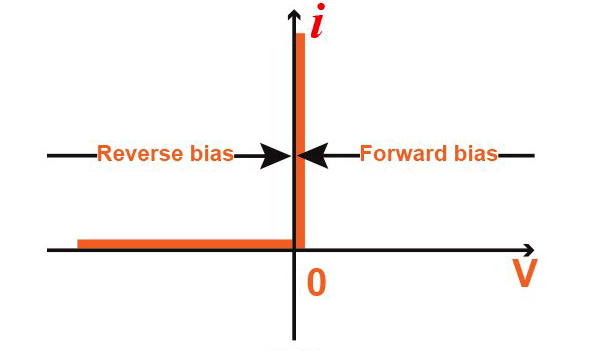
\includegraphics[scale=.4]{ideal-diode.png}
\centering \linebreak \linebreak Figure 2.1.0: 
\end{figure}

 \hfill \break \break \break

\textbf{\textit{\Large {"The characteristics of an ideal diode are those of a switch that can conduct current in only one direction." [1] }}} \hfill \break

\end{multicols}

One of the important parameters for the diode is the resistance at the point or region of operation. If we consider the conduction region defined by the direction of \textbf{\textit{i}} and polarity of \textbf{\textit{V}} in Fig. 2.1.0, we will find that the value of the forward resistance, R\_F, as defined by Ohm’s law is:

\begin{equation}
R_{F} = \frac{V_{F}}{ I_{F}} = \frac{0 V}{(1, 2, ..., n) A} = 0 \Omega
\end{equation}

where $V_F$ is the forward voltage across the diode and $I_F$ is the forward current through the diode. \hfill \break \break

\textbf{\textit{\Large {"The ideal diode, therefore, is a short circuit for the region of conduction." [1] }}} \hfill \break

Consider the region of negatively applied potential (third quadrant) of Figure 2.1.0:

\begin{equation}
R_{R} = \frac{V_{R}}{ I_{R}} = \frac{(-1, -2,..., -n)V}{0mA} = \infty \Omega
\end{equation}

where $V_R$ is reverse voltage across the diode and $I_R$ is reverse current in the diode.

\hfill \break \break

\textbf{\textit{\Large {"The ideal diode, therefore, is an open circuit in the region of non-conduction." [1] }}} \hfill \break

\pagebreak

In review, the conditions depicted in Figure. 2.1.1 are applicable.

\begin{figure}[H]
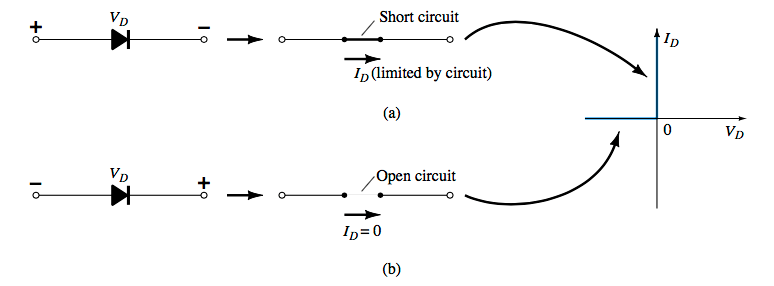
\includegraphics[scale=.6]{3.png}
\centering \linebreak \linebreak Figure 2.1.1: (a) Conduction and (b) non-conduction states of the ideal diode as determined by the applied bias.
\end{figure}

\subsection{Reverse Bias Condition ( Vd $<$ 0V ):}

Assuming that, if a diode has two parts a p-material as anode and a n-material as cathode, then, if an external potential of V volts is applied across the p-n junction such that the positive terminal is connected to the n-type material and the negative terminal is connected to the p-type material as shown in Figure 2.2.0, the number of uncovered positive ions in the depletion region of the n-type material will increase due to the large number of “free” electrons drawn to the positive potential of the applied voltage. For similar reasons, the number of uncovered negative ions will increase in the p-type material. The net effect, therefore, is a widening of the depletion region. This widening of the depletion region will establish too great a barrier for the majority carriers to overcome, effectively reducing the majority carrier flow to zero as shown in Figure 2.2.0.

\begin{figure}[H]
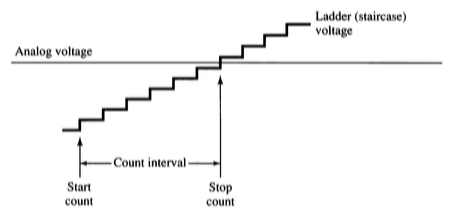
\includegraphics[scale=.8]{4.png}
\centering \linebreak \linebreak Figure 2.2.0: Reverse-biased  p-n junction.
\end{figure}

\textbf{\textit{\Large {"The current that exists under reverse-bias conditions is called the reverse sat- uration current and is represented by I$_{s}$." [1] }}}

\pagebreak

\subsection{Forward Bias Condition ( Vd $>$ 0V ):}

A forward-bias or “on” condition is established by applying the positive potential to the p-type material and the negative potential to the n-type material as shown in Figure 2.3.0. For future reference, therefore:

\begin{figure}[H]
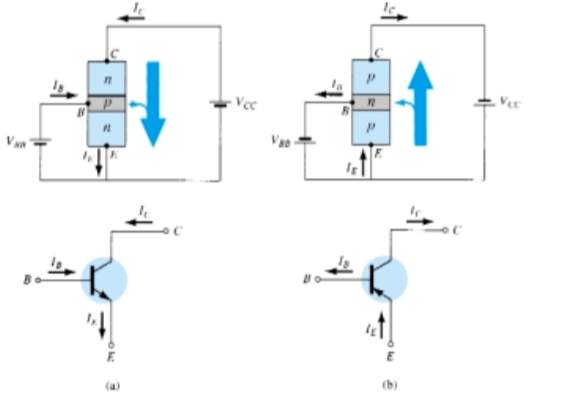
\includegraphics[scale=.8]{5.png}
\centering \linebreak \linebreak Figure 2.3.0: Forward-biased  p-n junction.
\end{figure}

The application of a forward-bias potential VD will “pressure” electrons in the n-type material and holes in the p-type material to recombine with the ions near the boundary and reduce the width of the depletion region as shown in Figure 2.3.0. 

\begin{multicols}{2}
The resulting minority-carrier flow of electrons from the p-type material to the n-type material (and of holes from the n-type material to the p-type material) has not changed in magnitude (since the conduction level is controlled primarily by the limited number of impurities in the material), but the reduction in the width of the depletion region has resulted in a heavy majority flow across the junction. An electron of the n-type material now “sees” a reduced barrier at the junction due to the reduced depletion region and a strong attraction for the positive potential applied to the p-type material. As the applied bias increases in magnitude the depletion region will continue to decrease in width until a flood of electrons can pass through the junction, resulting in an exponential rise in current as shown in the forward-bias region of the characteristics of Figure 2.3.1. Note that the vertical scale of Figure 2.3.1 is measured in milliamperes (although some semiconductor diodes will have a vertical scale measured in amperes) and the horizontal scale in the forward-bias region has a maximum of 1 V. Typically, therefore, the voltage across a forward-biased diode will be less than 1 V. Note also, how quickly the current rises beyond the knee of the curve. \linebreak \linebreak

\begin{figure}[H]
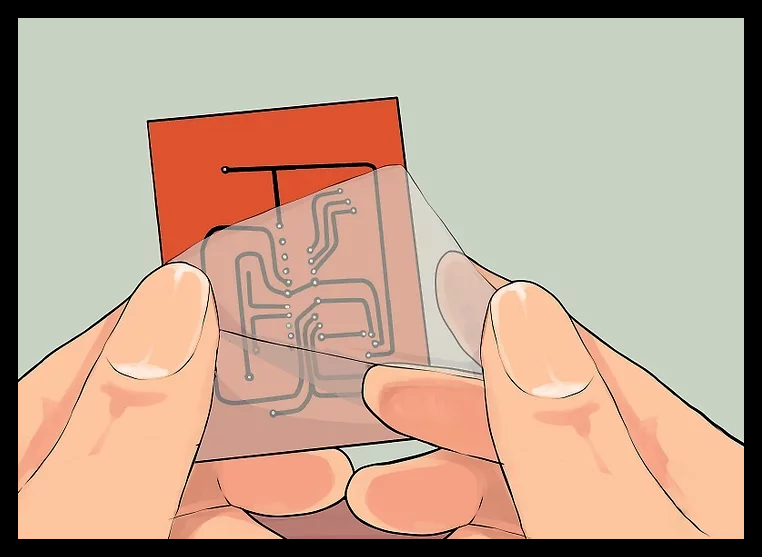
\includegraphics[scale=.45]{6.png}
\centering \linebreak \linebreak Figure 2.3.1: Silicon semiconductor diode characteristics.
\end{figure}
\end{multicols}

It can be demonstrated through the use of solid-state physics that the general characteristics of a semiconductor diode can be defined by the following equation for the forward- and reverse-bias regions:

\textbf{\textit{\Large {
\begin{equation}
I = I_{s} ( e^\frac{qV}{mKt} - 1 ) 
\end{equation}
}}}

\pagebreak

\subsection{Zener Region:}

Even though the scale of Figure 2.3.1 is in tens of volts in the negative region, there is a point where the application of too negative a voltage will result in a sharp change in the characteristics, as shown in Figure 2.4.0 The current increases at a very rapid rate in a direction opposite to that of the positive voltage region. The reverse-bias potential that results in this dramatic change in characteristics is called the Zener potential and is given the symbol V$_{Z}$. \hfill \break 

As the voltage across the diode increases in the reverse-bias region, the velocity of the minority carriers responsible for the reverse saturation current Is will also increase. Eventually, their velocity and associated kinetic energy $W_{k} = \frac{1}{2} mv^2 $ will be sufficient to release additional carriers through collisions with otherwise stable atomic structures. That is, an ionization process will result whereby valence electrons absorb sufficient energy to leave the parent atom. These additional carriers can then aid the ionization process to the point where a high avalanche current is established and the avalanche breakdown region determined.

\begin{figure}[H]
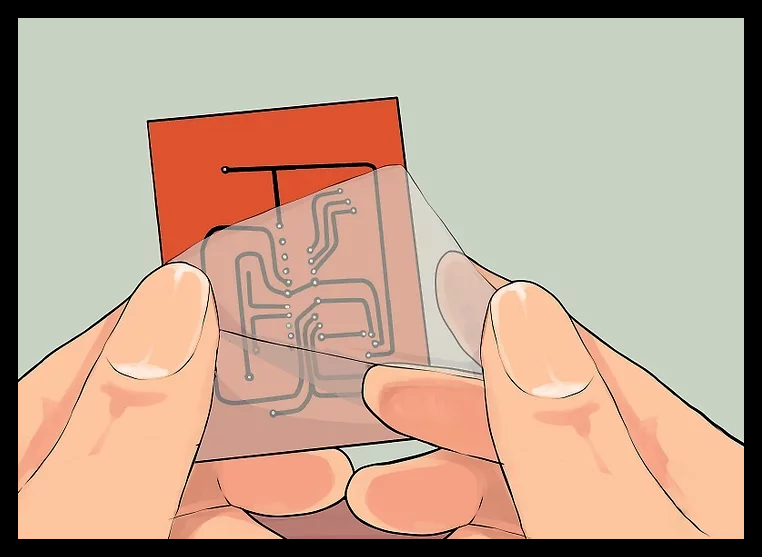
\includegraphics[scale=.45]{6.png}
\centering \linebreak \linebreak Figure 2.4.0: Zener Region.
\end{figure}

The avalanche region (V$_{Z}$) can be brought closer to the vertical axis by increasing the doping levels in the p- and n-type materials. However, as V$_{Z}$ decreases to very low levels, such as  5 V, another mechanism, called Zener breakdown, will contribute to the sharp change in the characteristic. It occurs because there is a strong electric field in the region of the junction that can disrupt the bonding forces within the atom and “generate” carriers. Although the Zener breakdown mechanism is a significant contributor only at lower levels of V$_{Z}$, this sharp change in the characteristic at any level is called the Zener region and diodes employing this unique portion of the characteristic of a p-n junction are called Zener diodes. \hfill \break

The Zener region of the semiconductor diode described must be avoided if the response of a system is not to be completely altered by the sharp change in characteristics in this reverse-voltage region. \hfill \break \break

\textbf{\textit{\Large {"The maximum reverse-bias potential that can be applied before entering the Zener region is called the peak inverse voltage (referred to simply as the PIV rating) or the peak reverse voltage (denoted by PRV rating)." [1] }}}

\pagebreak

\section{Development:}

The practice consist in two steps:

\begin{itemize}
\item Measure the forward and reverse voltage of several diodes.
\item Measure the current of the same diodes applying a define amount of voltage to have an idea of how the characteristic curve looks like.
\end{itemize}

\subsection{Forward and Reverse Bias Voltage:}

In first place, before analyzing the characteristic curve, we measure the polarization voltage of each diode. To have a forward-biased  diode circuit it's necessary to connect the positive terminal of the source (voltage source, VOM, etc) to the anode -In LED's this terminal it's more larger than the other- and the negative terminal to the cathode. This will allow the diode to behave like a closed circuit as long as the threshold voltage (barrier potential) it's reached.

\begin{figure}[H]
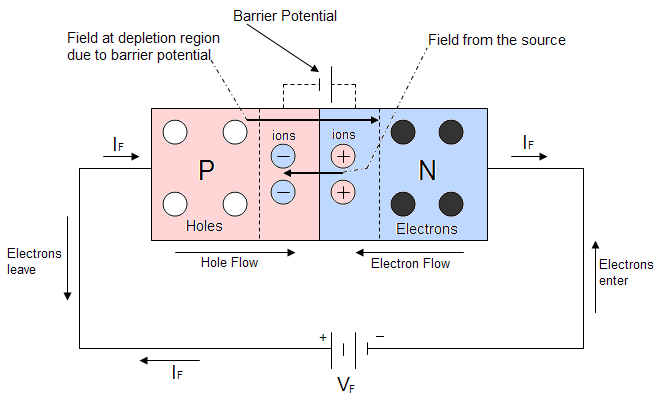
\includegraphics[scale=.55]{forward-biased.png}
\centering \linebreak Figure 3.1.0: Forward-biased diode circuit.
\end{figure}

On the other hand it's necessary to measure the reverse-biased diode circuit by connecting the negative terminal of the source to the anode, and the positive to the cathode terminal. This will allow the diode to behave like a open circuit.

\begin{figure}[H]
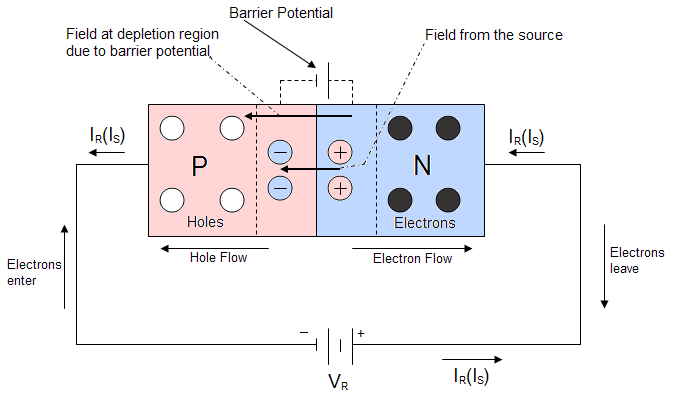
\includegraphics[scale=.55]{reverse-biased.png}
\centering \linebreak Figure 3.1.1: Reverse-biased diode circuit.
\end{figure}

After analyzing both behaviors we make a table with our results highlighting 6 different diodes: 1N4003, 1N4148, red LED, Green LED, white LED and infrared LED. 

\subsubsection{Forward Bias Voltage Table:}

According to the image 3.1.1.0, we connect each diode to the VOM and register the diode voltage:

\begin{multicols}{2}

\begin{figure}[H]
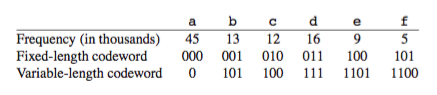
\includegraphics[scale=.5]{1.png}
\centering \linebreak \linebreak Figure 3.1.1.0: VOM forward diode connection.
\end{figure}

\begin{center}
\begin{tabular}[.5cm]{l c c }
\toprule
Diode & Diode Voltage \\
\midrule
1N4003 & 0.55 V \\
\cmidrule{1-2}
1N4148 & 0.38 V \\
\cmidrule{1-2}
Red LED & 1.33 V \\
\cmidrule{1-2}
Green LED & 1.8 V \\
\cmidrule{1-2}
White LED & 2.4 V \\
\cmidrule{1-2}
IR LED & 1.03 V \\
\bottomrule
\linebreak
\end{tabular}
\end{center} 

\end{multicols}

\subsubsection{Reverse Bias Voltage Table:}

According to the image 3.1.2.0, we connect each diode to the VOM and register the diode voltage:

\begin{multicols}{2}

\begin{figure}[H]
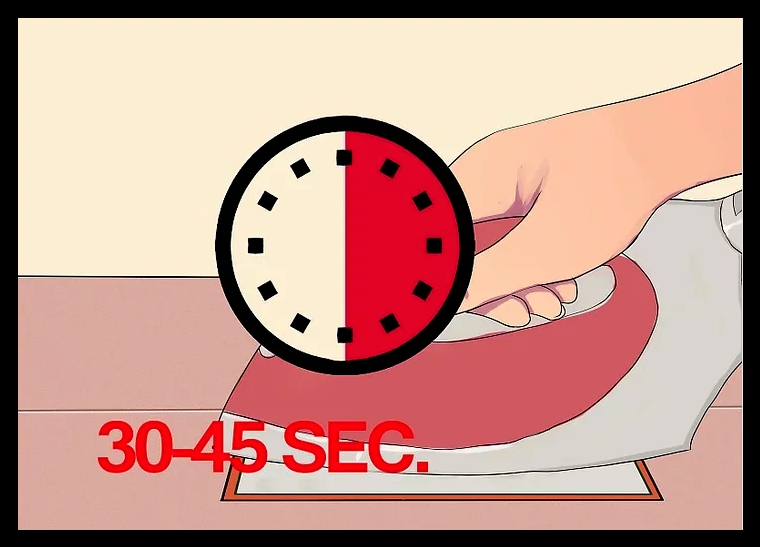
\includegraphics[scale=.5]{2.png}
\centering \linebreak \linebreak Figure 3.1.2.0: VOM reverse diode connection.
\end{figure}

\begin{center}
\begin{tabular}[.5cm]{l c c }
\toprule
Diode & Diode Voltage \\
\midrule
1N4003 & OL V \\
\cmidrule{1-2}
1N4148 & OL V \\
\cmidrule{1-2}
Red LED & OL V \\
\cmidrule{1-2}
Green LED & OL V \\
\cmidrule{1-2}
White LED & OL V \\
\cmidrule{1-2}
IR LED & OL V \\
\bottomrule
\linebreak
\end{tabular}
\end{center} 

\end{multicols}

\pagebreak

\subsection{Diode Characteristic Curve:}

We assemble the circuit in the figure 3.2.0, then variating the source voltage, we measure the current and capture all the information in the following table:

\begin{center}
\begin{tabular}[.5cm]{l c c c c c c c }
\toprule
Voltage [ V ] & 1N4003 & 1N4148 & Red LED & Green LED & Blue LED & IR LED \\
\midrule
0.0 V & 0.0 A & 0.0 A & 0.0 A & 0.0 A & 0.0 A & 0.0 A \\
\cmidrule{1-7}
0.2 V & 0.028 $\mu$A & 126.4 $\mu$A & 0.002 $\mu$A & 0.002 $\mu$A & 0.002 $\mu$A & 0.0 A \\
\cmidrule{1-7}
0.4 V & 0.209 $\mu$A & 348.9 $\mu$A & 0.002 $\mu$A & 0.002 $\mu$A & 0.002 $\mu$A & 0.0 A \\
\cmidrule{1-7}
0.6 V & 0.546 mA & 0.98 mA & 0.002 $\mu$A & 0.002 $\mu$A & 0.002 $\mu$A & 0.0 A \\
\cmidrule{1-7}
0.8 V & 0.07 A & 46.8 mA & 0.002 $\mu$A & 0.002 $\mu$A & 0.002 $\mu$A & 0.012 $\mu$A \\
\cmidrule{1-7}
1.0 V & 1.56 A & 120.5 mA & 0.05 $\mu$A & 0.002 $\mu$A & 0.002 $\mu$A & 0.5 $\mu$A \\
\cmidrule{1-7}
1.2 V & 4.49 A & 238 mA & 2.41 $\mu$A & 0.004 $\mu$A & 0.002 $\mu$A & 0.200 mA \\
\cmidrule{1-7}
1.4 V & 7.68 A & 388.4 mA & 10.8 $\mu$A & 0.009 $\mu$A & 0.002 $\mu$A & 1.24 mA \\
\cmidrule{1-7}
1.6 V & 12.7 A & 496.2 mA & 100 $\mu$A & 2.41 $\mu$A & 0.002 $\mu$A & 2.8 mA \\
\cmidrule{1-7}
1.8 V & 16.4 A & 583.1 mA & 0.81 mA & 311 $\mu$A & 0.03 $\mu$A & 4.9 mA \\
\cmidrule{1-7}
2.0 V & 18.3 A & 668.4 mA & 2.13 mA & 1.49 mA & 0.35 $\mu$A & 195 mA \\
\cmidrule{1-7}
2.2 V & - & - & 3.4 mA & 2.8 mA & 0.83 $\mu$A & 350.8 mA \\
\cmidrule{1-7}
2.4 V & - & - & 116.8 mA & 4.5 mA & 19.5 $\mu$A & 528.6 mA \\
\cmidrule{1-7}
2.6 V & - & - & - & - & 133.3 $\mu$A & - \\
\cmidrule{1-7}
2.8 V & - & - & - & - & 0.7 mA & - \\
\cmidrule{1-7}
3.0 V & - & - & - & - & 1.8 mA & - \\
\bottomrule
\linebreak
\end{tabular}
\end{center} 

{\bfseries\itshape Observation:} {\itshape The only values that are similar with our simulations it's for the diodes 1N4003, 1N4148, IR-LED, for some reason, in the simulation the LEDs red, green and blue, have the same values, a lot different for the practical measuring.} 

\begin{figure}[H]
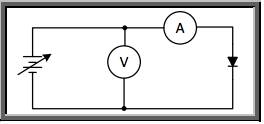
\includegraphics[scale=1.6]{circuit.png}
\centering \linebreak \linebreak Figure 3.2.0: Diode Circuit.
\end{figure}

\pagebreak

After measure, and capturing the information in the table, we put the values in a specialized software. And graphic {\bfseries\itshape Voltage [ V ]} against {\bfseries\itshape Current [ A ]}. 

\begin{multicols}{2}
\begin{figure}[H]
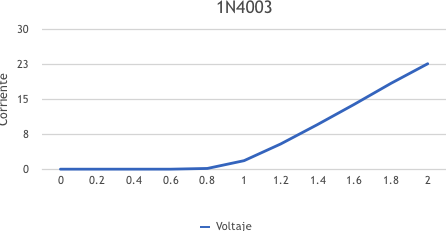
\includegraphics[scale=.44]{1N4003-GRAPH-DIODE.png}
\centering \linebreak \linebreak Figure 3.2.0: 1N4003 diode characteristic curve (Laboratory values).
\end{figure}

\begin{figure}[H]
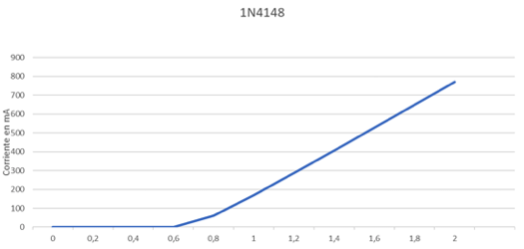
\includegraphics[scale=.4]{1N4148-GRAPH-DIODE.png}
\centering \linebreak \linebreak Figure 3.2.1: 1N4148 diode characteristic curve (Laboratory values).
\end{figure}
\end{multicols}

\begin{multicols}{2}
\begin{figure}[H]
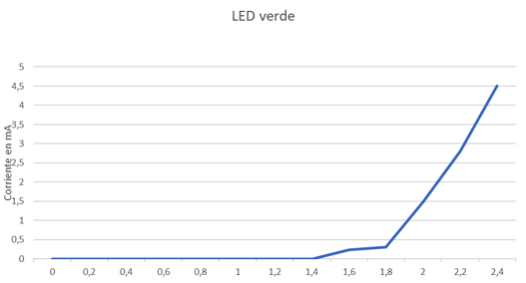
\includegraphics[scale=.4]{GREEN-GRAPH.png}
\centering \linebreak \linebreak Figure 3.2.2: Green LED characteristic curve (Laboratory values).
\end{figure}

\begin{figure}[H]
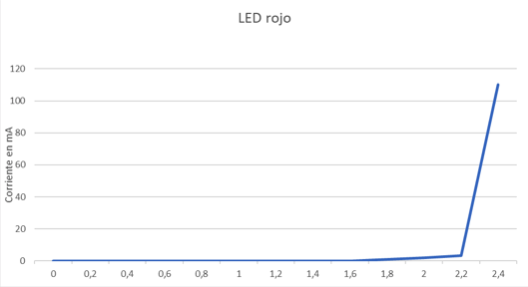
\includegraphics[scale=.4]{RED-GRAPH-DIODE.png}
\centering \linebreak \linebreak Figure 3.2.3: Red LED characteristic curve (Laboratory values).
\end{figure}
\end{multicols}

\begin{multicols}{2}
\begin{figure}[H]
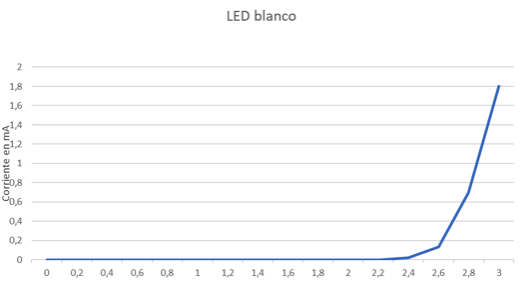
\includegraphics[scale=.4]{WHITE-GRAPH.png}
\centering \linebreak \linebreak Figure 3.2.4: White LED characteristic curve (Laboratory values).
\end{figure}

\begin{figure}[H]
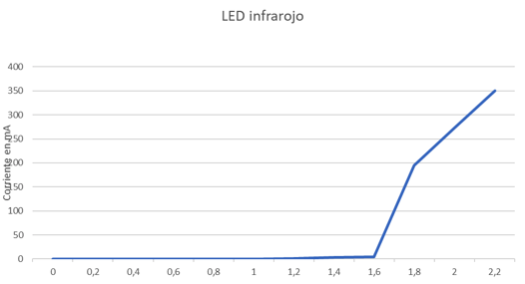
\includegraphics[scale=.4]{IR-LED.png}
\centering \linebreak \linebreak Figure 3.2.5: IR LED characteristic curve (Laboratory values).
\end{figure}
\end{multicols}

\pagebreak

\section{Simulations:}

The simulation are realized in Proteus and Multisim.

\subsection{Forward and Reverse Bias Voltage Simulation:}

For some reason, for the forward-biased voltage of the LED's diodes, Multisim recognize the circuit as and open one, the same for the reverse-biased, so we only put the forward-biased simulations for the diode 1N4003 and 1N4148, as we know, in reverse-biased all diodes will "imitate" an open circuit, so we believe that it's enough only putting one.

\begin{figure}[H]
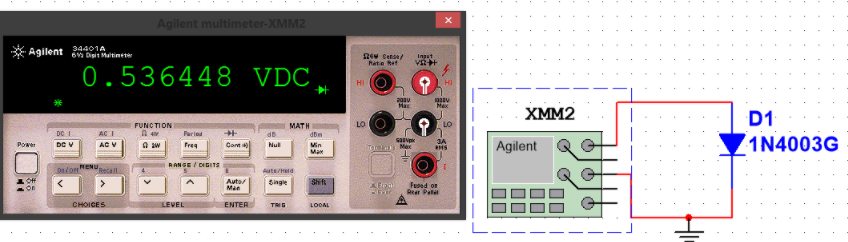
\includegraphics[scale=.6]{1N4003.png}
\centering \linebreak \linebreak Figure 4.1.0: Simulation of a forward-biased 1N4003-Diode.
\end{figure}

\begin{figure}[H]
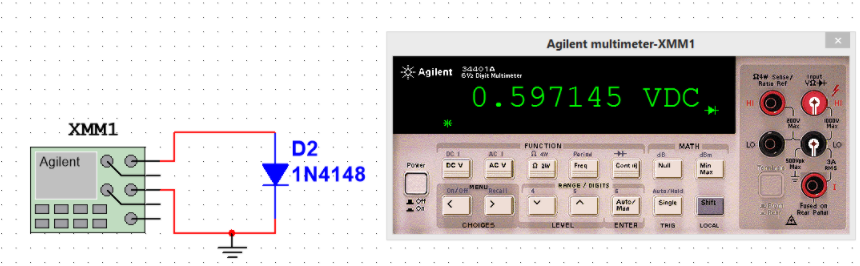
\includegraphics[scale=.6]{1N4148.png}
\centering \linebreak \linebreak Figure 4.1.1: Simulation of a forward-biased 1N4148-Diode.
\end{figure}

\begin{figure}[H]
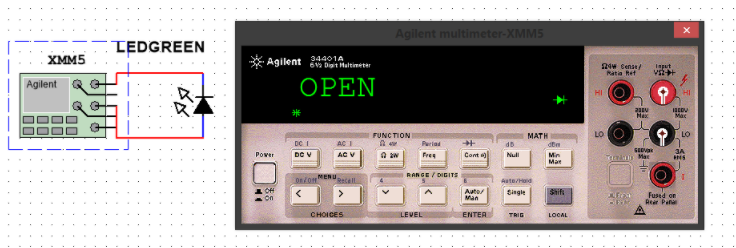
\includegraphics[scale=.6]{OPEN.png}
\centering \linebreak \linebreak Figure 4.1.2: Simulation of a inverse-biased Green-Diode.
\end{figure}

\pagebreak

\subsection{Characteristic Curve of a Diode Simulation:}

We simulate each diode and capture the characteristic curve. Proteus and Multisim doesn't have a white LED so we decide to use a blue LED instead.

\subsubsection{1N4003 Simulation:}

1N4003 diode graph and simulation.

\begin{figure}[H]
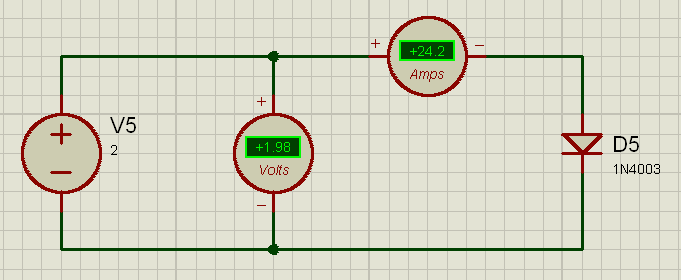
\includegraphics[scale=.68]{sim1N4003.png}
\centering \linebreak \linebreak Figure 4.2.1.0 (a): 1N4003 simulation.
\end{figure}

\begin{figure}[H]
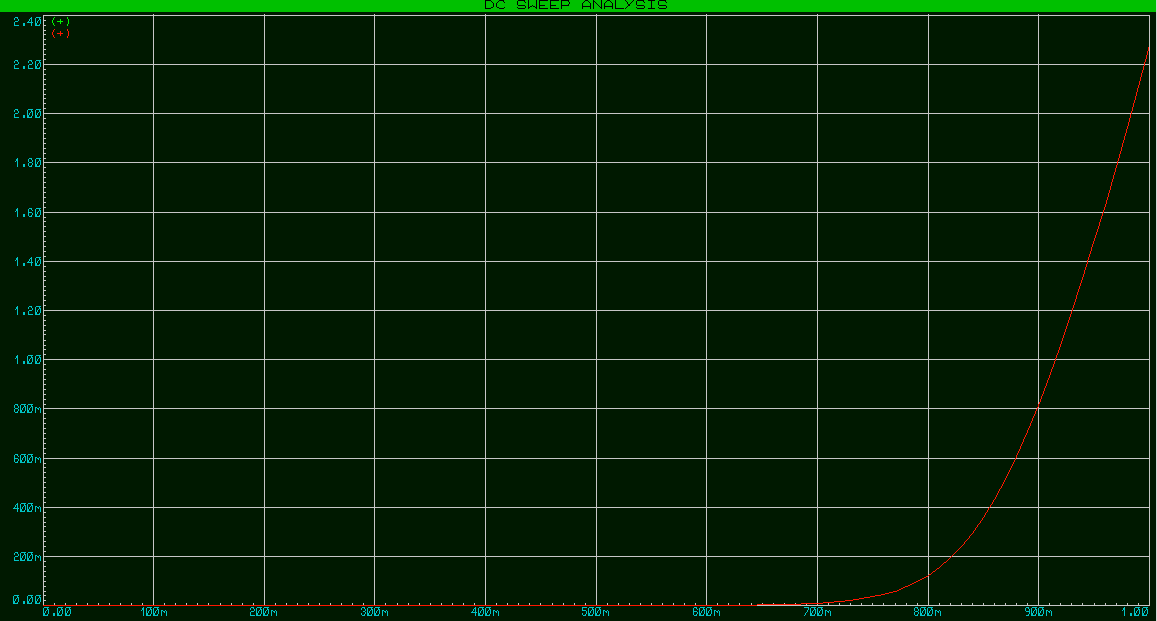
\includegraphics[scale=.4]{1N4003-GRAPH.png}
\centering \linebreak \linebreak Figure 4.2.1.0 (b): 1N4003 graph.
\end{figure}

\pagebreak

\subsubsection{1N4148 Simulation:}

1N4148 diode graph and simulation.

\begin{figure}[H]
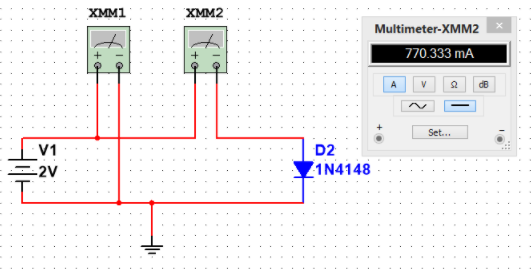
\includegraphics[scale=.85]{sim1N4148.png}
\centering \linebreak \linebreak Figure 4.2.2.0 (a): 1N4148 simulation.
\end{figure}

\begin{figure}[H]
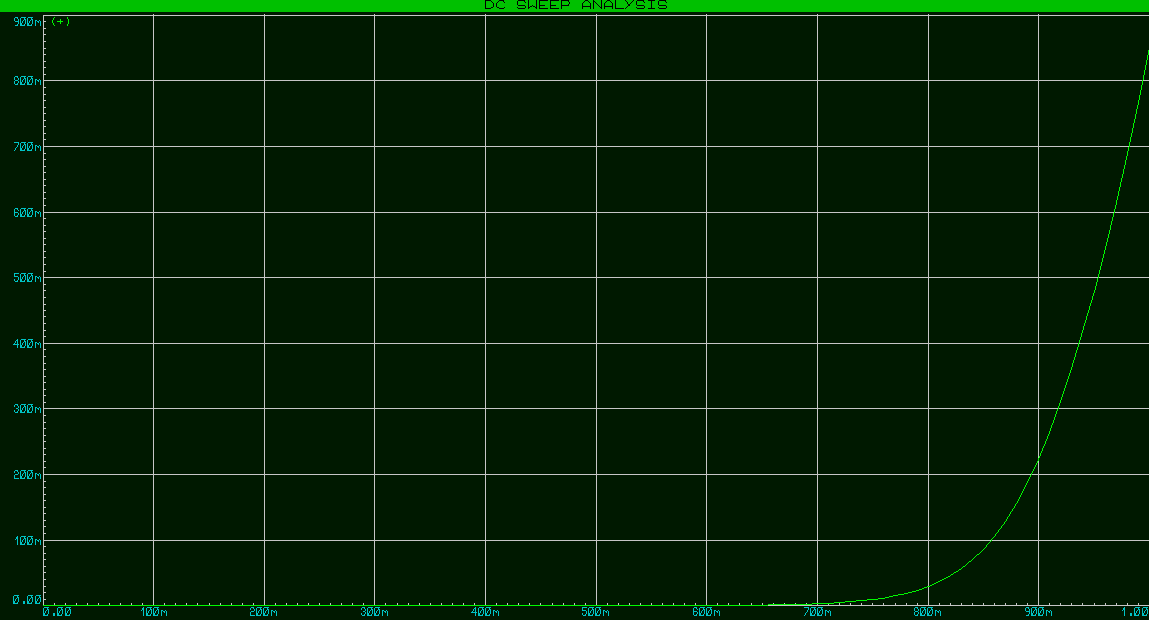
\includegraphics[scale=.4]{1N4148-GRAPH.png}
\centering \linebreak \linebreak Figure 4.2.2.0 (b): 1N4148 graph.
\end{figure}

\pagebreak

\subsubsection{Red LED Simulation:}

Red LED graph and simulation.

\begin{figure}[H]
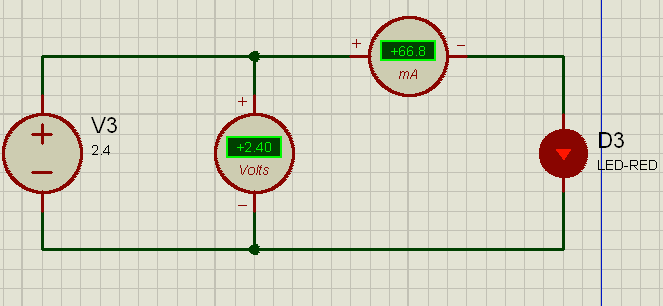
\includegraphics[scale=.68]{simRED.png}
\centering \linebreak \linebreak Figure 4.2.3.0 (a): Red LED simulation.
\end{figure}

\begin{figure}[H]
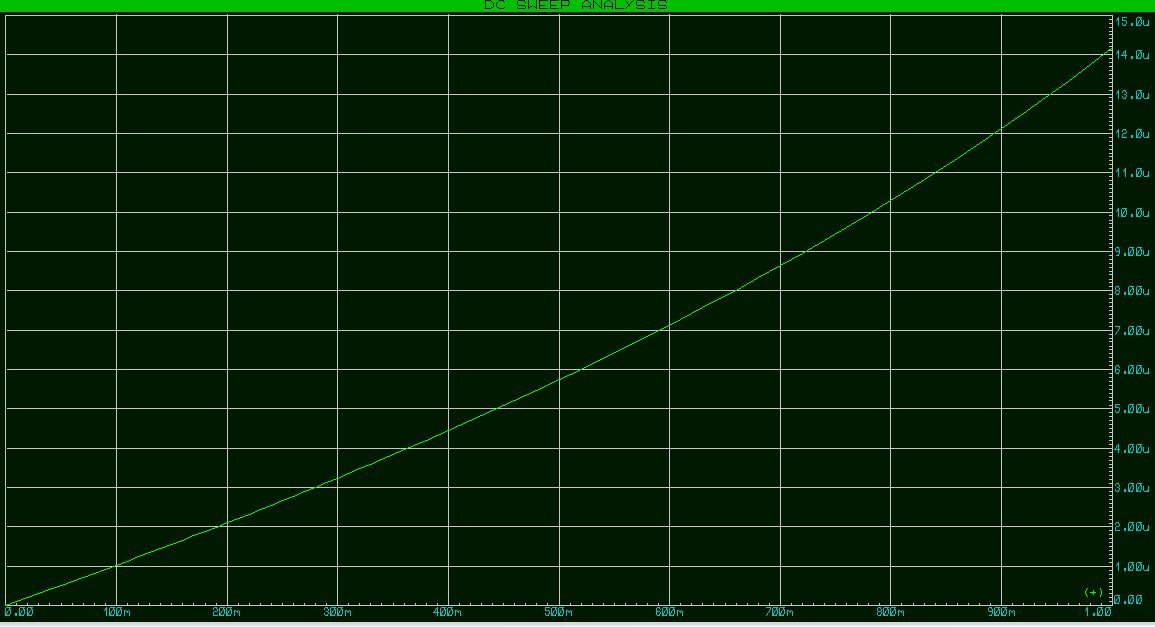
\includegraphics[scale=.4]{RED-GRAPH.png}
\centering \linebreak \linebreak Figure 4.2.3.0 (b): Red LED graph.
\end{figure}

\pagebreak

\subsubsection{Green LED Simulation:}

Green LED graph and simulation.

\begin{figure}[H]
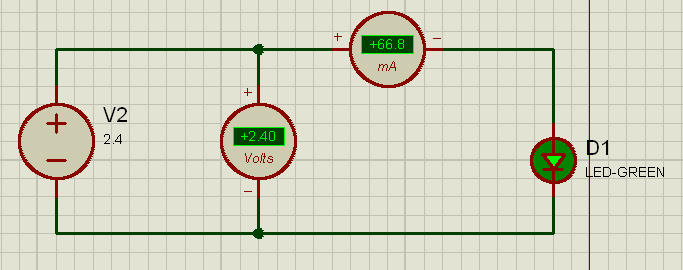
\includegraphics[scale=.68]{simGREEN.png}
\centering \linebreak \linebreak Figure 4.2.4.0 (a): Green LED simulation.
\end{figure}

\begin{figure}[H]
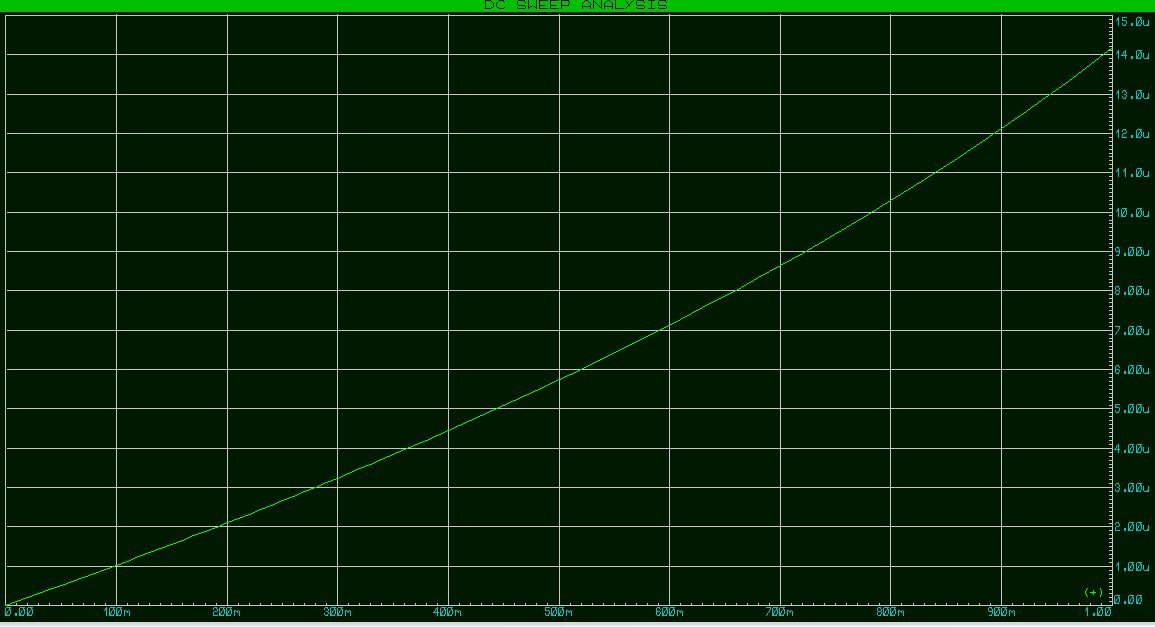
\includegraphics[scale=.4]{RED-GRAPH.png}
\centering \linebreak \linebreak Figure 4.2.4.0 (b): Green LED graph.
\end{figure}

\pagebreak

\subsubsection{Blue LED Simulation:}

Blue LED graph and simulation.

\begin{figure}[H]
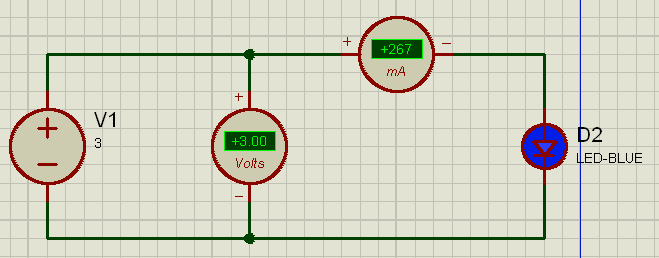
\includegraphics[scale=.68]{simBLUE.png}
\centering \linebreak \linebreak Figure 4.2.5.0 (a): Blue LED simulation.
\end{figure}

\begin{figure}[H]
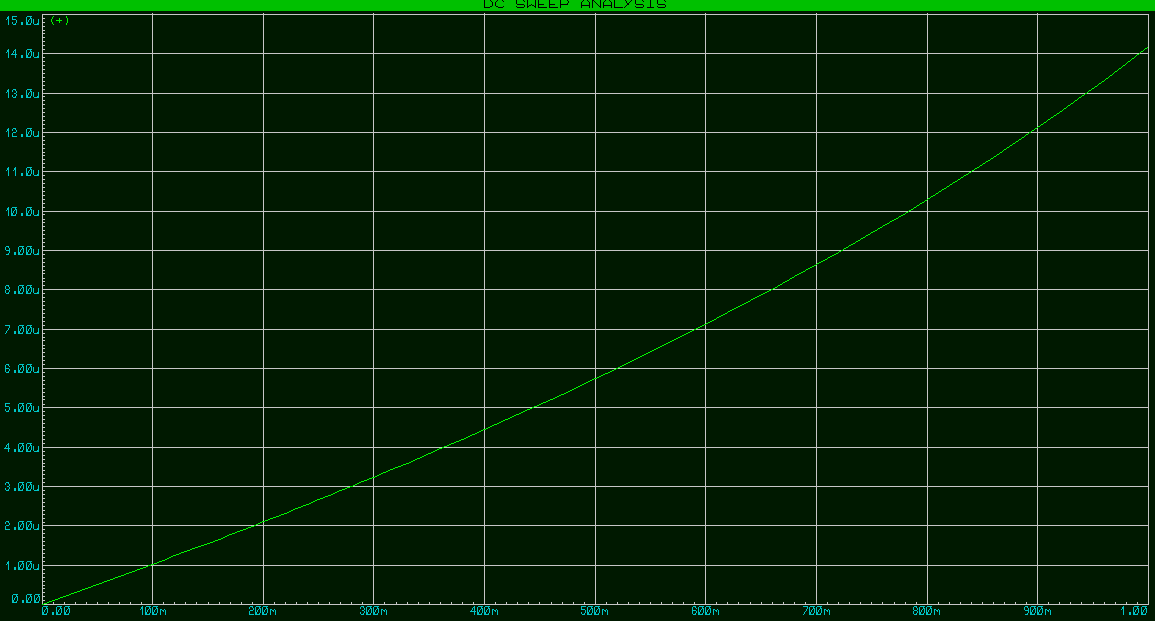
\includegraphics[scale=.4]{BLUE-GRAPH.png}
\centering \linebreak \linebreak Figure 4.2.5.0 (b): Blue LED graph.
\end{figure}

\pagebreak

\subsubsection{IR LED Simulation:}

IR LED graph and simulation.

\begin{figure}[H]
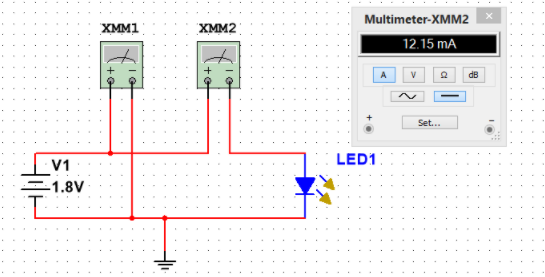
\includegraphics[scale=.85]{simIR.png}
\centering \linebreak \linebreak Figure 4.2.6.0 (a): IR LED simulation.
\end{figure}

\begin{figure}[H]
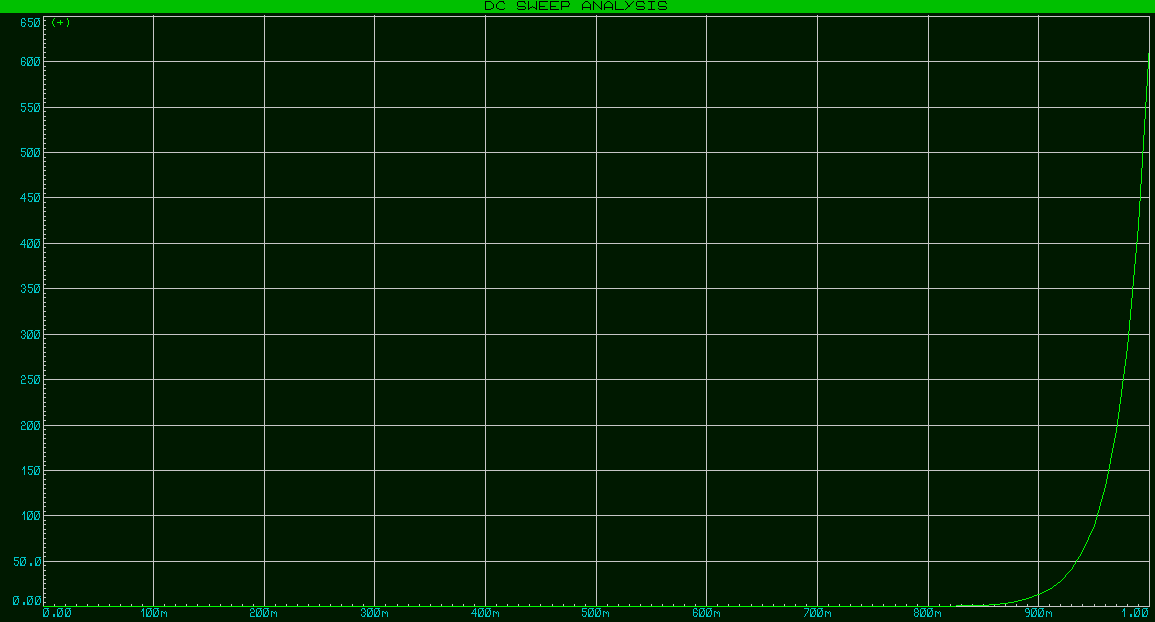
\includegraphics[scale=.4]{IR-GRAPH.png}
\centering \linebreak \linebreak Figure 4.2.6.0 (b): IR LED graph.
\end{figure}

\pagebreak

\section{Simulation Tables:}

After simulating with Proteus and Multisim, we capture the data on the following tables:

\subsection{Forward and Reverse Bias Voltage Table:}

\begin{multicols}{2}
\begin{center}
\begin{tabular}[.5cm]{l c c }
\toprule
Diode & Diode Voltage \\
\midrule
1N4003 & 0.53 V \\
\cmidrule{1-2}
1N4148 &  0.59 V \\
\cmidrule{1-2}
Red LED & OPEN \\
\cmidrule{1-2}
Green LED & OPEN \\
\cmidrule{1-2}
White LED & OPEN \\
\cmidrule{1-2}
IR LED & OPEN \\
\bottomrule
\linebreak
\end{tabular}
\centering \linebreak \linebreak Table 5.1.0: Forward-biased simulation table.
\end{center} 

\begin{center}
\begin{tabular}[.5cm]{l c c }
\toprule
Diode & Diode Voltage \\
\midrule
1N4003 & OPEN \\
\cmidrule{1-2}
1N4148 & OPEN \\
\cmidrule{1-2}
Red LED & OPEN \\
\cmidrule{1-2}
Green LED & OPEN \\
\cmidrule{1-2}
White LED & OPEN \\
\cmidrule{1-2}
IR LED & OPEN \\
\bottomrule
\linebreak
\end{tabular}
\centering \linebreak \linebreak Table 5.1.1: Reverse-biased simulation table.
\end{center} 
\end{multicols}

{\bfseries\itshape Observation:} {\itshape For some reason Proteus as Multisim measure an open circuit for forward and inverse polarization of the LED's (Go to section 4.1 to see the simulation).}

\subsection{Characteristic Curve of a Diode Table:}

Comparing Voltage against Current of each diode to visualize how the characteristic curve of a diode looks like (Results of the curve are in the section 4.2): 

\begin{center}
\begin{tabular}[.5cm]{l c c c c c c c }
\toprule
Voltage [ V ] & 1N4003 & 1N4148 & Red LED & Green LED & Blue LED & IR LED \\
\midrule
0.0 V & 0.0 A & 0.0 A & 0.0 A & 0.0 A & 0.0 A & 0.0 A \\
\cmidrule{1-7}
0.2 V & 0.0 $\mu$A & 227.5 $\mu$A & 2.1 $\mu$A & 2.1 $\mu$A & 2.1 $\mu$A & 0.0 A \\
\cmidrule{1-7}
0.4 V & 0.0 $\mu$A & 560.6 $\mu$A & 4.45 $\mu$A & 4.45 $\mu$A & 4.45 $\mu$A & 0.0 A \\
\cmidrule{1-7}
0.6 V & 0.0 mA & 1.19 mA & 7.13 $\mu$A & 7.13 $\mu$A & 7.13 $\mu$A & 0.0 A \\
\cmidrule{1-7}
0.8 V & 0.16 A & 61.2 mA & 10.3 $\mu$A & 10.3 $\mu$A & 10.4 $\mu$A & 0.002 $\mu$A \\
\cmidrule{1-7}
1.0 V & 1.83 A & 169.7 mA & 19.2 $\mu$A & 19.2 $\mu$A & 14 $\mu$A & 0.005 $\mu$A \\
\cmidrule{1-7}
1.2 V & 5.42 A & 286 mA & 22.6 $\mu$A & 22.6 $\mu$A & 19.2 $\mu$A & 0.114 mA \\
\cmidrule{1-7}
1.4 V & 9.57 A & 405.7 mA & 26.3 $\mu$A & 26.3 $\mu$A & 26.3 $\mu$A & 0.243 mA \\
\cmidrule{1-7}
1.6 V & 13.9 A & 526.4 mA & 37.3 $\mu$A & 37.3 $\mu$A & 37.3 $\mu$A & 0.556 mA \\
\cmidrule{1-7}
1.8 V & 18.4 A & 648.1 mA & 58.5 $\mu$A & 58.5 $\mu$A & 58.5 $\mu$A & 12.1 mA \\
\cmidrule{1-7}
2.0 V & 22.3 A & 770.3 mA & 120 $\mu$A & 120 $\mu$A & 120 $\mu$A & 560.6 mA \\
\cmidrule{1-7}
2.2 V & - & - & 2.84 mA & 2.84 mA & 2.84 mA & - \\
\cmidrule{1-7}
2.4 V & - & - & 66.8 mA & 66.8 mA & 66.8 mA & - \\
\cmidrule{1-7}
2.6 V & - & - & - & - & 133.3 mA & - \\
\cmidrule{1-7}
2.8 V & - & - & - & - & 200 mA & - \\
\cmidrule{1-7}
3.0 V & - & - & - & - & 257.5 mA & - \\
\bottomrule
\linebreak
\end{tabular}
\end{center} 

{\bfseries\itshape Observation:} {\itshape Note that we change the white diode for a blue one in the simulation because we didn't find it in Proteus or Multisim.}

\pagebreak

\section{Questionnaire:}

\begin{itemize}
\item {\bfseries\itshape What is the principle of operation of a diode?}

Allows the circulation of the electric current through it in one direction.
When a positive voltage is applied to the 'P' side and a negative side 'N', the electrons on the 'N' side are pushed to the 'P' side and the electrons flow through the material 'P' beyond the Limits of the diode. Similarly the voids in the material 'P' are pushed with a negative voltage to the side of the material 'N' and the voids flow through the material 'N'. In the opposite case, when a positive voltage is applied to the side 'N' and a negative side 'P', the electrons on the 'N' side are pushed to the 'N' side and the 'P' side holes are pushed Next to 'P'. In this case the electrons in the diode do not move and consequently there is no current

\item {\bfseries\itshape What does the diode voltage represent?}

Represents the voltage required to pass the "potential barrier" to the electron flow, as long as the voltage does not exceed 0.3 V in the case of germanium or 0.7 V in the case of silicon, there will be no current flow

\item {\bfseries\itshape Mention the most important applications of the diode:}
\begin{itemize}
\item Rectifier: The diodes can be used to rectify alternating current signals and convert them to positive or negative currents of direct current with the help of inductance. These are called rectifiers

\item Voltage multiplier: A voltage multiplier is made with diodes and with capacitors, it serves to increase the input voltage in a multiplicative way. The more meshes there are, the more voltage will be.

\item Voltage limiter: It allows us to transform a signal by manipulating it to vary its type (square or triangular), or its peak or peak-to-peak voltage values

\item Logical gates: It is possible to develop the logic gates with diodes that serve to provide a logical output response according to a type of input signal, you can make the logic gate "or" and type "and", the two are based on one Square continuous source
\end{itemize}

\item {\bfseries\itshape Mention to what is due to the diode voltage variation in the diodes:}
It is due to the potential barrier, this depends on element you use, germanium and silicon.
The direct diode characteristic is also affected by temperature,
Most important effect the influence on the potential barrier. As the
Temperature, the direct voltage needed to polarize the diode decreases


\item {\bfseries\itshape Mention why when the the diode voltage in direct bias is measured, the diode
turns on, however, the voltmeter does not show any reading:}

It lights up because current is flowing through the diode and it behaves like a closed circuit, but the voltmeter does not detect voltage because even though it injects a small amount of voltage, this does not measure potential difference because there is no resistance in series that gives us that voltage drop, to measure the voltage, we would have to connect another voltmeter in parallel.
\end{itemize}

\pagebreak

\section{Conclusions:}

As now we know, the diode has two forms of bias, forward and reverse, this gave us an idea how the electrons of the atoms inside the n-type and p-type behave. We prove that a positive terminal in the p-type and the negative to the n-type allows us to work with a forward-biased circuit. when ever the source voltage its bigger than the threshold voltage inside the diode. The diode has a lot of applications in the industry, one of them it's the construction of a voltage multiplier, this circuit is used for the generation of the high voltage required in the cathode ray tubes (like our old T.Vs). This device its one of the most important electronic devices, and for sure we'll still be work with it in the future. 


\pagebreak

\section{Bibliographic References:}

[ 1 ] BOYLESTAD, Robert L. "Electronic Devices and Circuit Theory". Edit. Prentice Hall. 2009.

\end{document}